\documentclass{report}
\usepackage{graphicx}

\author{Trinh Thanh Vinh}

\begin{document}
\title{Labwork 3: CUDA}
\maketitle
\section{Introduction}
This labwork is about using CUDA to fastly convert RGB images to grayscale. The main goal is to understand how to use GPU for parallel processing and to compare the performance of CPU and GPU implementations.
\section{Implementation}
In this labwork, I used the NVIDIA GeForce RTX 3060 GPU, which has 28 multiprocessors and a total of 3584 CUDA cores. The compute capability of this device is 8.6, and it has a total memory of 12.0 GiB. The device was selected using the \texttt{numba.cuda} library, which allows for easy access to CUDA devices in Python. The GPU implementation of the RGB to grayscale conversion was done using a CUDA kernel that processes each pixel in parallel. Each thread computes the grayscale value for one pixel by averaging the red, green, and blue components.

The CPU I used is 12th Gen Intel(R) Core(TM) i5-12400F (2.50 GHz). The CPU has 6 cores and 12 threads, with a base frequency of 2.50 GHz and a maximum turbo frequency of 4.40 GHz. The CPU has a total cache size of 18 MB and supports DDR4 memory with a maximum speed of 3200 MHz. To convert the RGB image to grayscale on the CPU, I implemented a simple loop that iterates through each pixel and computes the grayscale value by averaging the red, green, and blue components.

The expected result is that the GPU implementation will be significantly faster than the CPU implementation due to the parallel processing capabilities of the GPU.
\section{Results}
The results of the experiment show while both methods produce the same output, the GPU implementation is significantly faster than the CPU implementation. The GPU processed the image in about 0.00012 seconds, while the CPU took nearly 1.2 seconds to complete the same task. This demonstrates the power of parallel processing and the advantages of using GPUs for tasks that can be parallelized, such as image processing.

The Figure \ref{fig:gpu-output} shows the comparison of the results from the CPU and GPU implementations. The output images are identical, confirming that both methods produce the same result, but the performance difference is significant, with the GPU implementation being much faster.

\begin{figure}[ht]
    \centering
    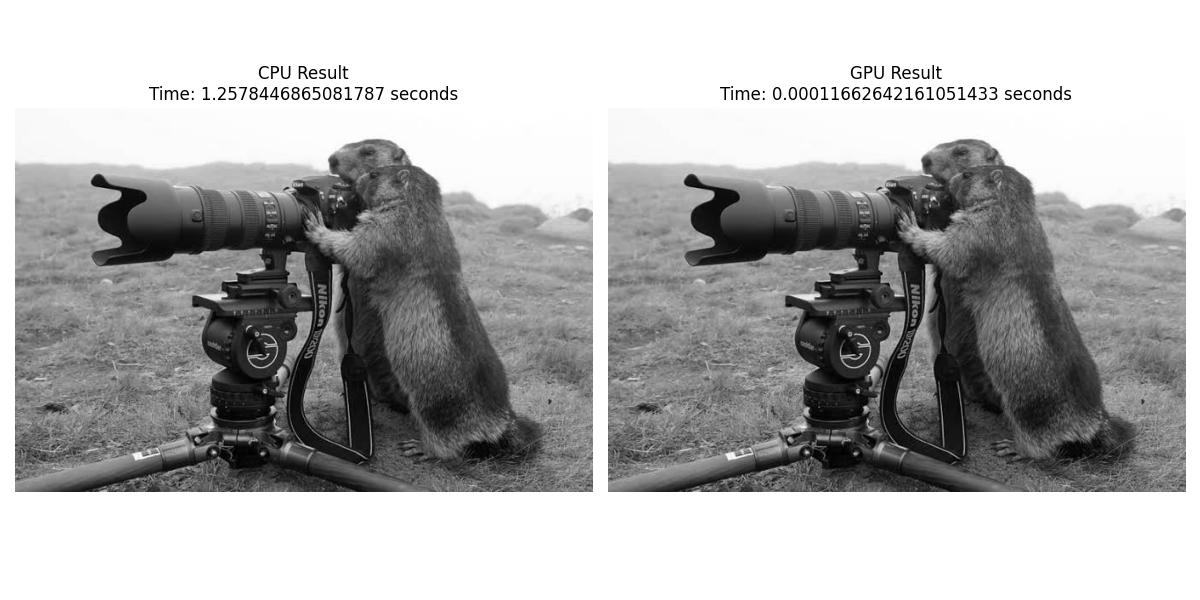
\includegraphics[width=\textwidth]{result.jpg}
    \caption{Comparison of the results from the CPU and GPU implementations}
    \label{fig:gpu-output}
\end{figure}
\end{document}